% !TEX root = paper.tex
\section{Evaluation}

LSD is evaluated against 12 C and C++ benchmarks in the LLVM Compiler
Infrastructure (version 5.0.2). The benchmarks are selected from previous
automatic DOALL parallelization papers~\cite{johnson:12:pldi,kim:12:cgo}. We
exclude benchmarks for lack of a FORTRAN front-end, duplicate behavior, or no
significant Spec-DOALL coverage exhibiting.

The machine is using a 28-core (56 threads with hyperthreading) Intel(R) Xeon(R)
CPU E5-2697 v3 CPU running at 2.60GHz (turbo-boost disabled) with 756GB of
memory. The operating system is Ubuntu 16.04.5 LTS with GCC 5.5 (version 5.5.0
20171010).


\subsection{Parallelization Performance}
Figures Needed:
\begin{itemize}
\item General Speed Plot: With different cores (1-28), all benchmarks
\item Speedup Comparison: 24 cores performance compared with Privateer
Runtime breakdown (how to minimize the overhead?)

\end{itemize}

\begin{figure*}[htp]
  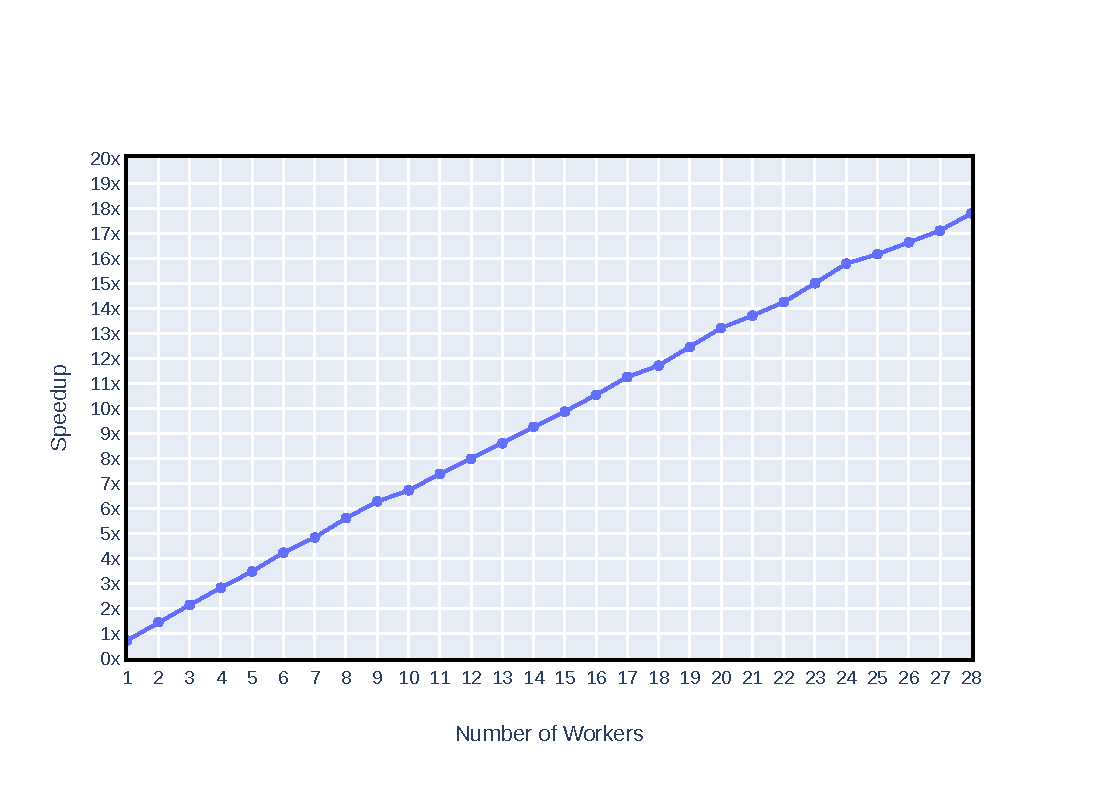
\includegraphics[width=\textwidth]{figures/3mm-scale-crop}
  \caption{3mm Speedup over Different Numbers of Workers}
  \label{fig:3mm-scale}
\end{figure*}

\subsubsection{Effect of parallelization on vectorization}

instrumentation kills vectorization


\subsection{Static Analysis and Enablers}
Figures Needed:
\begin{itemize}
\item CAF: with and without; no topping; with only BasicLoopAA and ScevAA
\item Coverage: Spec-DOALL percentage of coverage of each benchmark
\item Enablers: Enablers used for each benchmark
\item Optimization level: Performance with different optimization levels
\end{itemize}

Discussion Needed:


\subsection{Overhead Breakdown}

\begin{figure*}[htp]
  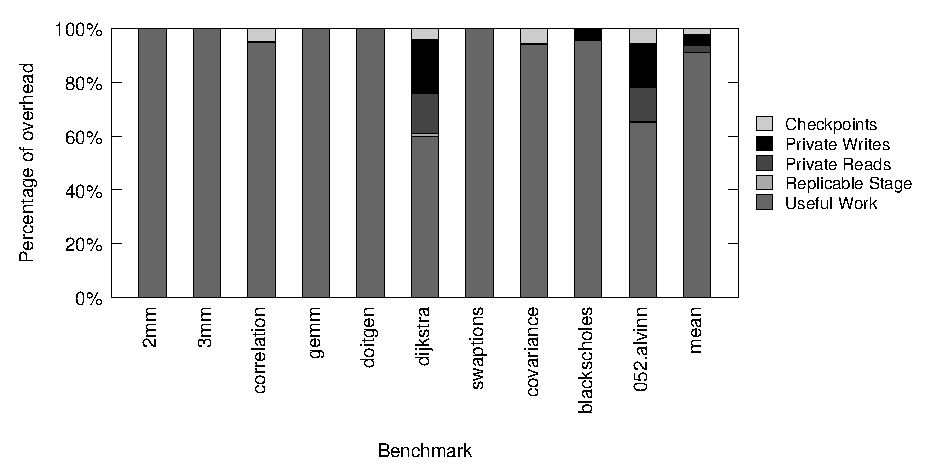
\includegraphics[width=0.9\textwidth]{figures/overheads}
\end{figure*}

\subsection{Power Consumption}

Power and energy stats here

